\documentclass[11pt]{beamer}
\usetheme{Warsaw}
\usepackage[utf8]{inputenc}
\usepackage[spanish]{babel}
\usepackage{amsmath}
\usepackage{amsfonts}
\usepackage{amssymb}
\usepackage{graphicx}
\author{N.Pérez-Medina}
\title{Capítulo 15 - \textbf{Modelado de Datos}}
\setbeamercovered{transparent} 
\setbeamertemplate{navigation symbols}{} 
\logo{
\includegraphics[scale=0.04]{logo_fing_uach_bn.png} } 
\institute{\textbf{FING - UACH}
	\\
	\begin{small}
	\textit{Resumen del libro 'Recetas Numéricas en C' de H. Press}\\
	\end{small}
	
	\bigskip
	
	\begin{small}
	\textbf{Catedrático:} Dr. José Luis Herrera Aguilar
	\end{small}		
	} 
\date{\today} 


% Para tener un morado coqueto
\definecolor{lightPurple}{RGB}{186, 146, 209} % Morado claro
\definecolor{darkPurple}{RGB}{98, 54, 150}    % Morado oscuro
\setbeamercolor{structure}{fg=darkPurple} % Color principal para estructuras
\setbeamercolor{frametitle}{bg=darkPurple, fg=white} % Título del marco
\setbeamercolor{block title}{bg=darkPurple, fg=white} % Título de bloques
\setbeamercolor{block body}{bg=lightPurple!30, fg=black} % Cuerpo de bloques

\begin{document}

\begin{frame}
\maketitle
\end{frame}

\begin{frame}
\tableofcontents
\end{frame}

\section{Introducción}
\begin{frame} 
\tableofcontents[currentsection] % Solo muestra la sección actual
\end{frame}

\subsection{Ideas generales}
\begin{frame}{Ideas generales}
\begin{block}{Planteamiento central}
Dado un conjunto de observaciones, se desea ''resumir'' los datos ajustándolos a un \textbf{\textit{Modelo}} que depende de \textit{Parámetros Ajustables}
\end{block}


\begin{block}{Enfoque básico}
\begin{enumerate}
\item Se diseña una \textit{Función de Méritos}
\item Los \textit{Parámetros Ajustables} se ajustan para alcanzar el mínimo de la \textit{Función de Méritos}
\end{enumerate}
\end{block}
\end{frame}

\subsection{Pregunta fundamental}
\begin{frame}{Pregunta fundamental}
Una ves ajustados los \textit{Parámetros Ajustables}
\begin{block}{Intentamos responder}
\centering
\textit{''¿Estamos seguros de que no hay un ajuste \textbf{mucho mejor}?''}
\end{block}
\centering

\includegraphics[scale=0.7]{pregunta.jpeg} 
\end{frame}

\section{Mínimos Cuadrados como un Estimador de Máxima Verosimilitud}
\begin{frame} 
\tableofcontents[currentsection] % Solo muestra la sección actual
\end{frame}

\subsection{Sobre la Verosimilitud}
\begin{frame}{\textit{Sensación Intuitiva}}
\begin{block}{Planteamiento}
\small
Supongamos que ajustamos $N$ puntos de datos de la forma $(x_i,y_i), i = 1,\dots,N$, a un \textbf{\textit{Modelo}} que tiene $M$ \textit{Parámetros Ajustables} $a_j,j=1,\dots,M$. El \textbf{\textit{Modelo}} se expresa como

\begin{equation}
\hat{y}(x) = y(x;a_1,\dots,a_M)
\end{equation}

\end{block}

\begin{block}{Pregunta Fundamental}
\centering
\textit{''¿Estamos seguros de que no hay un ajuste \textbf{mucho mejor}?''}
\end{block}

\end{frame}

\begin{frame}{\textit{Sensación Intuitiva}}
\begin{block}{Planteamiento}
\small
Supongamos que ajustamos $N$ puntos de datos de la forma $(x_i,y_i), i = 1,\dots,N$, a un \textbf{\textit{Modelo}} que tiene $M$ \textit{Parámetros Ajustables} $a_j,j=1,\dots,M$. El \textbf{\textit{Modelo}} se expresa como

\begin{equation}
\hat{y}(x) = y(x;a_1,\dots,a_M)
\end{equation}

\end{block}

\begin{block}{Pregunta Fundamental \textit{ajustada}}
\centering
\textit{''¿Qué tan probable es que los Parámetros Ajustables que determinamos hayan producido los datos observados?''}
\end{block}

\end{frame}

\begin{frame}{\textit{Sensación Intuitiva}}
\begin{block}{Planteamiento}
\small
Supongamos que ajustamos $N$ puntos de datos de la forma $(x_i,y_i), i = 1,\dots,N$, a un \textbf{\textit{Modelo}} que tiene $M$ \textit{Parámetros Ajustables} $a_j,j=1,\dots,M$. El \textbf{\textit{Modelo}} se expresa como

\begin{equation}
\hat{y}(x) = y(x;a_1,\dots,a_M)
\end{equation}

\end{block}

\begin{block}{Pregunta Fundamental \textit{más ajustada}}
\centering
\textit{''¿Qué tan probable es que los Parámetros Ajustables que determinamos hayan producido los datos observados \textbf{con errores}?''}
\end{block}

\end{frame}


\begin{frame}{\textit{Sensación Intuitiva}}
\begin{block}{Planteamiento}
\small
Supongamos que ajustamos $N$ puntos de datos de la forma $(x_i,y_i), i = 1,\dots,N$, a un \textbf{\textit{Modelo}} que tiene $M$ \textit{Parámetros Ajustables} $a_j,j=1,\dots,M$. El \textbf{\textit{Modelo}} se expresa como

\begin{equation}
\hat{y}(x) = y(x;a_1,\dots,a_M)
\end{equation}

\end{block}

\begin{block}{Pregunta Fundamental \textit{más ajustada}}
\centering
\textit{''¿Qué tan probable es que los Parámetros Ajustables que determinamos hayan producido los datos observados \textbf{con errores}?''}
\end{block}

\begin{block}{\textit{Estimación de Máxima Verosimilitud}}
Identificamos la probabilidad descrita como la \textbf{\textit{Verosimilitud}} de los \textit{Parametros Ajustables}
\end{block}

\end{frame}

\subsection{Sobre los Mínimos Cuadrados}
\begin{frame}{Los errores}
\begin{block}{Error aleatorio $\epsilon$}
Para cada conjunto de $M$ parámetros $a = \{ a_1,\dots,a_M \}$, el \textbf{\textit{Modelo}} determina un valor $\hat{y}(x)$ al que le \textit{''falta''} un error aleatorio $\epsilon_i$ para llegar a cada dato observado $y_i$
\end{block}
\centering
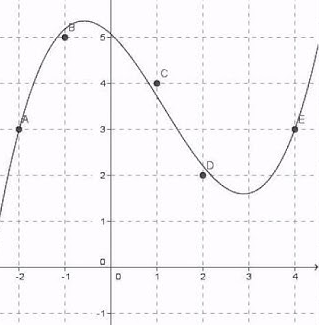
\includegraphics[scale=0.5]{errores-idea-grafica.png} 
\end{frame}

\begin{frame}{Los errores}

\begin{block}{\textbf{Modelo}}
\begin{equation}
y_i = \hat{y}(x_i;a_1,\dots,a_M) + \epsilon_i
\end{equation}
\end{block}
\begin{block}{Asumimos:}
Que la distribución de probabilidades de los errores sigue una \textbf{distribución normal}
\begin{equation}
p(\epsilon_i)=\frac{1}{\sqrt{2\pi}\sigma_i}e^{-\frac{\epsilon_i^2}{2\sigma_i^2}}
\end{equation}
\end{block}

\end{frame}

\begin{frame}{Ahora sí}
\begin{block}{Desarrollo}
Como $y_i = \hat{y}(x_i;a_1,\dots,a_M) + \epsilon_i$ entonces 
$$\epsilon_i = y_i - \hat{y}(x_i;a_1,\dots,a_M)$$
Luego, la probablidad de obtener un $y_i$ dado un conjunto de \textit{Parametros Ajustables} es 
$$ p(y_i|a_1,\dots,a_M)=\frac{1}{\sqrt{2\pi}\sigma_i}e^{-\frac{(y_i - \hat{y}(x_i;a_1,\dots,a_M))^2}{2\sigma_i^2}} $$
Entonces la probablidad de obtener los datos es el producto de las probabilidades de cada punto
$$ P \propto \prod_{i=1}^{N} \frac{1}{\sqrt{2\pi}\sigma_i}e^{-\frac{(y_i - \hat{y}(x_i;a_1,\dots,a_M))^2}{2\sigma_i^2}} $$
\end{block}
\end{frame}

\begin{frame}{Ahora sí}
\begin{block}{Desarrollo}
Maximizar esta expresión es equivalente a minimizar el negativo de su logaritmo, al que llamamos $\chi^2$
$$ \chi^2 \equiv \sum_{i=1}^{N} \frac{[y_i - \hat{y}(x_i)]^2}{\sigma_i^2} $$
Si las $\sigma_i$ no se conocen, pueden asumirse todas iguales. En general, minimizar $\chi^2$ es equivalente a minimizar 
$$ \sum_{i=1}^{N} [y_i - \hat{y}(x_i)]^2 $$
De ahi que entendamos a los \textbf{Mínimos Cuadrados como un Estimador de Máxima Verosimilitud}
\end{block}
\end{frame}

\subsection{Ajsute por Chi-Cuadrada $\chi^2$}
\begin{frame}{Sobre $\chi^2$}
\small
\begin{block}{En general}
La estimación de máxima \textbf{Verosimilitud} de los \textit{Parámetros Ajustables} del \textbf{Modelo} se obtiene minimizando la cantidad

\begin{equation}
\chi^2 \equiv \sum_{i=1}^{N} \left[ \frac{y_i - y(x_i; a_1 \ldots a_M)}{\sigma_i} \right]^2
\end{equation}
\end{block}

\begin{block}{Sus derivadas}

Si tomamos la derivada de $\chi^2$ con respecto a los parámetros $a_k$, obtenemos ecuaciones que deben cumplirse en el \textbf{\textit{mínimo}} chi-cuadrado,

\begin{equation}
0 = \sum_{i=1}^{N} \frac{[y_i - y(x_i)]}{\sigma_i^2}
\left( \frac{\partial y(x_i; \ldots a_k \ldots)}{\partial a_k} \right), \quad
k = 1, \ldots, M
\end{equation}
Esto es, en general, un conjunto de $M$ ecuaciones no lineales para los $M$ parámetros desconocidos $a_k$. 
\end{block}
\end{frame}

\section*{Gracias}
\begin{frame}{Por su atención}
\centering
\begin{Huge}
Gracias \\

\medskip

\end{Huge}

\includegraphics[scale=0.2]{matematica.jpg} 
\end{frame}
\end{document}